\documentclass{beamer}
\usetheme{AnnArbor}
\usecolortheme{crane}
\usepackage{graphicx}
\title{My first presentation in Beamer}
\author{slopezv2}
\date{\today}
\begin{document}
	\begin{frame}
		\maketitle
	\end{frame}

	\begin{frame}{Outline}
		\tableofcontents
	\end{frame}

	\section{Welcome}
	\begin{frame}[t]{Welcome}
		Welcome Everyone
	\end{frame}

	\section{Test}
	\begin{frame}[t]{Welcome}
		Welcome Everyone
	\end{frame}

	\section{Bird}
	\begin{frame}{Bird}
		\begin{figure}
			\centering
			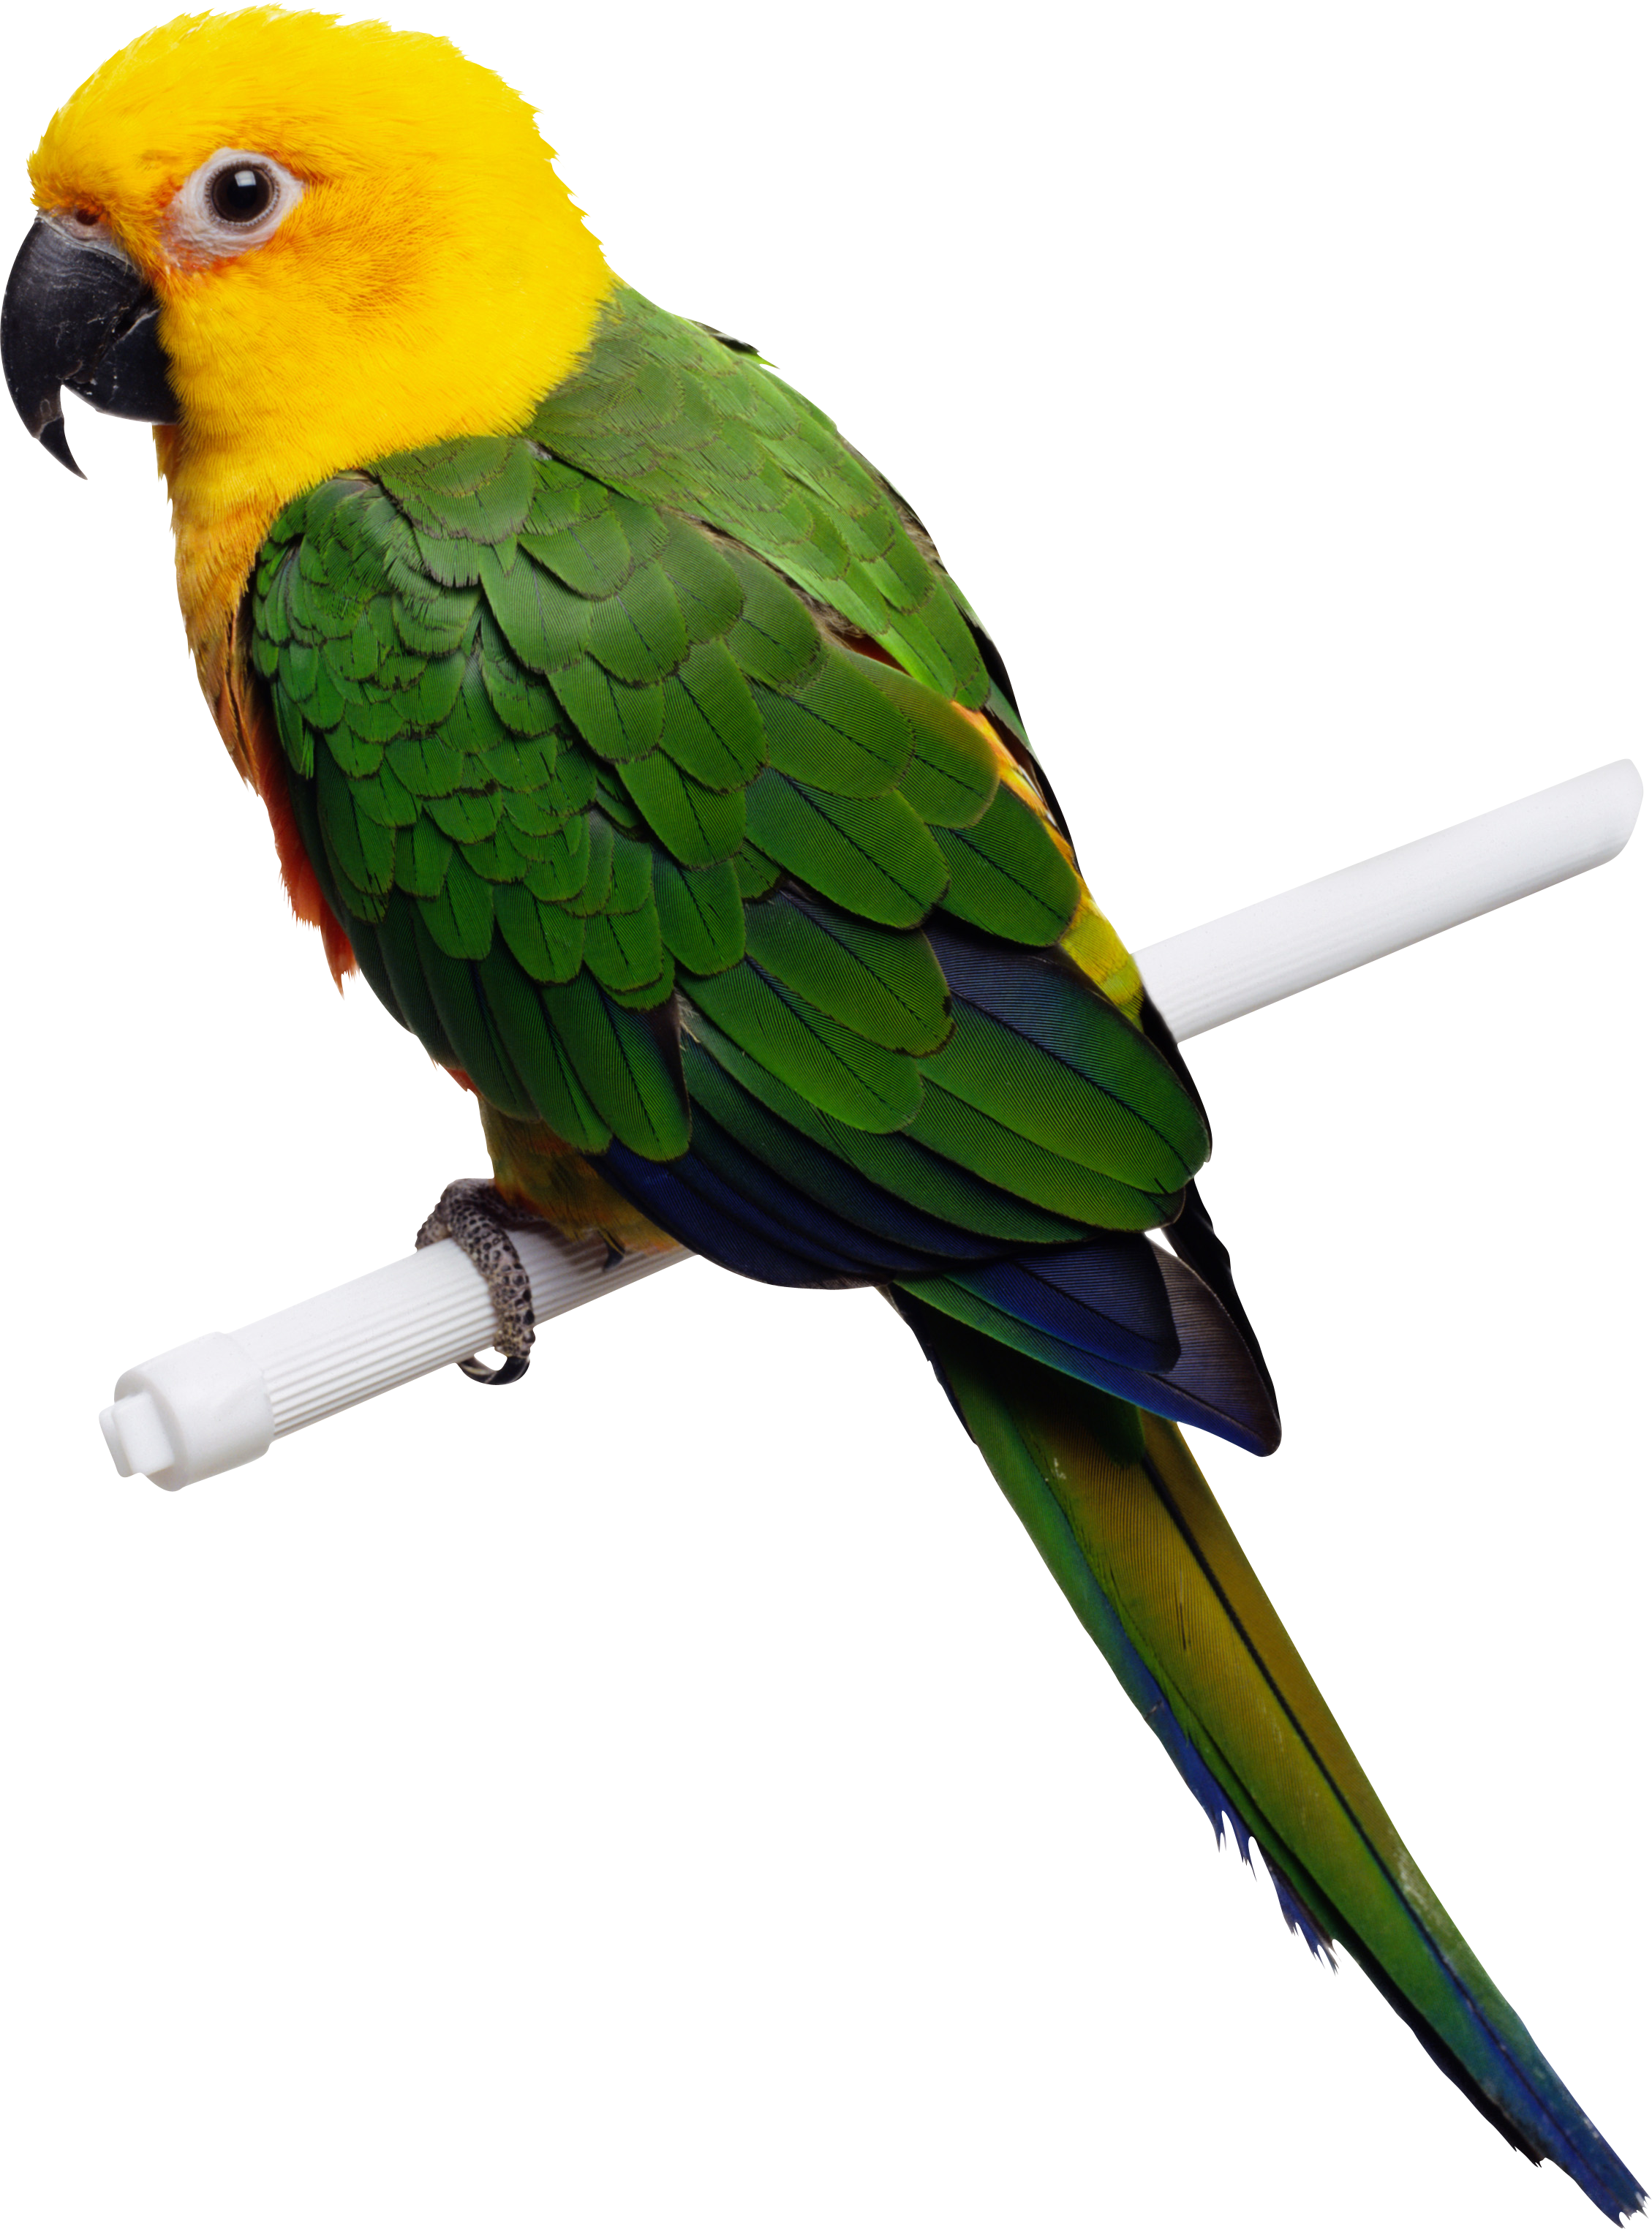
\includegraphics[width=3in]{parrot.png}
			\caption{Colorful Parrot}
		\end{figure}
	\end{frame}
	
	\section{Definitions}
	\begin{frame}{Definitions}
		\begin{table}
			\centering
			\begin{tabular}{clll}
				\hline
				No. & Item & Price & Code\\
				\hline
				1 & Note book & 10 & NB\\
				2 & Gel Pen & 40 & GP\\
				3 & Pencil & 5 & P\\
				4 & Wooden scale & 30 & WS\\
				\hline
			\end{tabular}
			\caption{Stationery Items}
		\end{table}
	\end{frame}

\end{document}